\documentclass[a4paper, twocolumn]{article}
\usepackage[pdftex, hidelinks,
            pdftitle={Report},
            pdfauthor={Erik S. Vasconcelos Jansson},
            pdfsubject={Report},
            pdfkeywords={report}]{hyperref}

\usepackage{bm}
\usepackage[T1]{fontenc}
\usepackage[utf8]{inputenc}
\usepackage{algorithmic}
\usepackage{algorithm}
\usepackage{amsfonts}
\usepackage{booktabs}
\usepackage{amssymb}
\usepackage{courier}
\usepackage{booktabs}
\usepackage{graphicx}
\usepackage{listings}
\usepackage{mathtools}
\lstset{basicstyle=\footnotesize\ttfamily,
        breakatwhitespace = false,
        breaklines = true,
        keepspaces = true,
        language = C++,
        showspaces = false,
        showstringspaces = false,
        belowcaptionskip = \bigskipamount,
        framerule = 0.80pt,
        frame = tb,
        numbers = left,
        belowskip = \bigskipamount,
        escapeinside={<@}{@>}}

\title{Introduction to Machine Learning \\
       Individual Laboration Report --3--}
\author{{Erik Sven Vasconcelos Jansson} \\
        {\href{mailto:erija578@student.liu.se}
        {\texttt{erija578@student.liu.se}}} \\
        {Linköping University, \, Sweden}}

\begin{document}
    \pagenumbering{arabic}
    \maketitle % Titles...

    \section*{Assignment 1}

        \begin{figure}[h!]
            \centering
            \caption{Sex Classifications of Australian Crabs}
            \label{fig:crabs}
            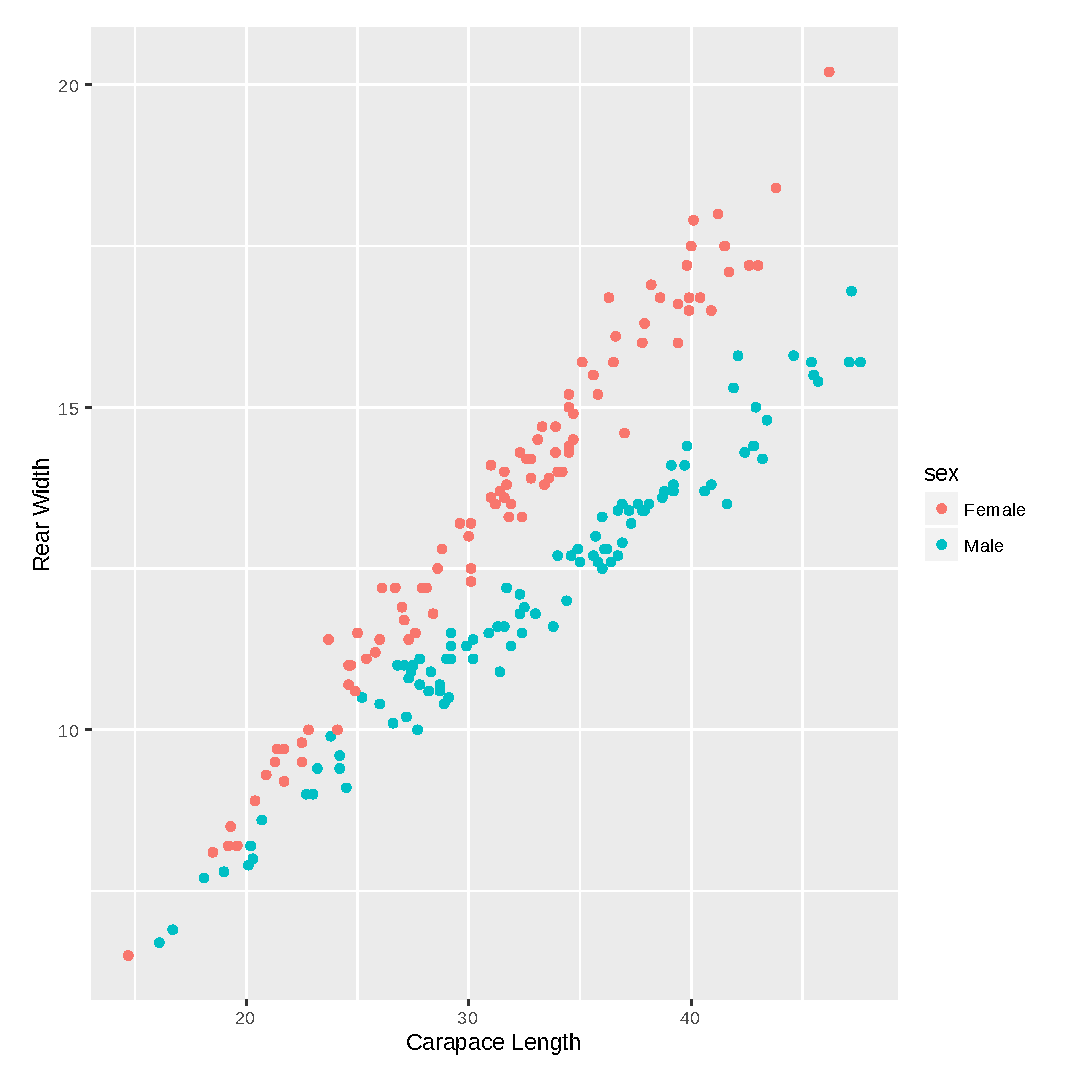
\includegraphics[width=0.5\textwidth]{share/crabs.eps}
        \end{figure}

        \begin{figure}[h!]
            \centering
            \caption{Decision Boundary for Australian Crabs}
            \label{fig:boundary}
            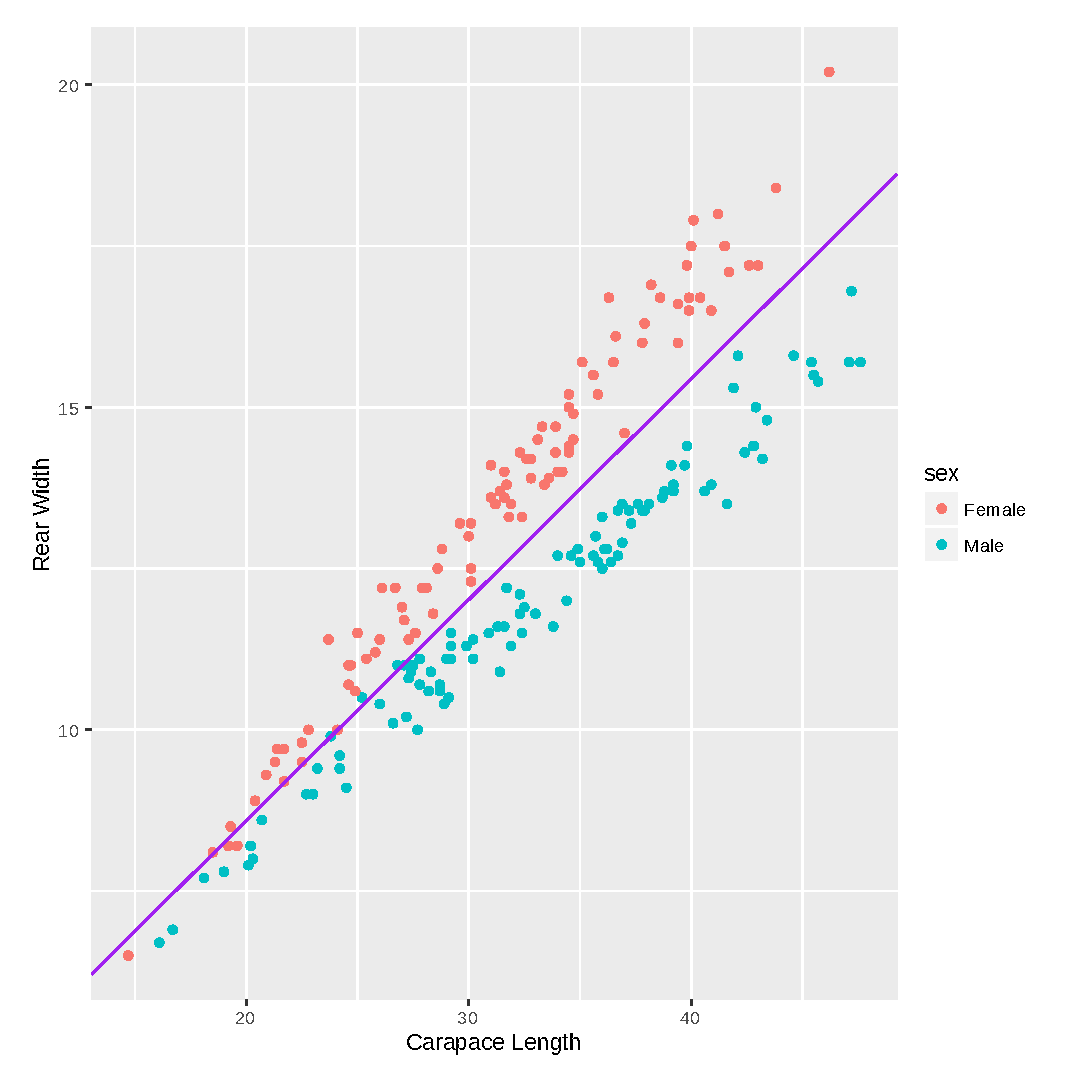
\includegraphics[width=0.5\textwidth]{share/boundary.eps}
        \end{figure}

        \begin{equation} \label{eq:lda}
        \begin{split}
            \hat{\pi}_k &= \frac{N_k}{N} \\
            \hat{\mu}_k &= \frac{1}{N_k}\sum_{i \in k}{\bm{x}_i} \\
            \Sigma_k &= \frac{1}{N_k}\sum_{i \in k}{(\bm{\hat{\mu}}_k - \bm{x}_i)(\bm{\hat{\mu}}_k - \bm{x}_i)^\intercal} \\
            \hat\Sigma &= \frac{1}{N}\sum_{k \in K}{N_k \Sigma_k} = \sum_{k \in K}{\frac{\mathrm{cov}\,X_k}{|X_k|}}
        \end{split}
        \end{equation}

        \begin{equation} \label{eq:weights}
        \begin{split}
            w_{k} &= \frac{\bm{\hat\mu}_k}{2}\hat\Sigma^{-1}\bm{\hat\mu}_k + \log\hat{\pi}_k \\
            \bm{w}_{k} &= \hat\Sigma^{-1}\bm{\hat\mu}_k
        \end{split}
        \end{equation}

    \section*{Assignment 2}

        ...

    \clearpage \nocite{*}
    \bibliographystyle{alpha}
    \bibliography{report}

    \onecolumn \appendix
    \section*{Appendix}

        ...

\end{document}
